\chapter{Storage Model for XML data}


The Extensible Markup Language (XML) is an
emerging standard for data representation and
exchange on the Internet.

\section{XML query language}

Several XML query languages were proposed including
Lorel [Abiteboul et al., 1997], XML QL
[Deutsch et al., 1999a], XML-GL [Ceri et al., 1999],
Quilt [Chamberlin et al., 2000], YATL
[Cluet et al., 1998], XPath [Clark and DeRose, 1999]
and XQuery [Chamberlin et al., 2001].
The surveys on XML schema languages
and query languages can be found in
[Bonifati and Ceri, 2000, Lee and Chu, 2000a].

\section{Persistent XML data storage model}

An XML document can be represented as a graph, Fig.\ref{fig:XML_graph}, or an
{\bf XML data graph}. Because elements of an XML document are ordered, in an XML
data graph, the
\begin{itemize}
  \item {\it ordinal} of an element is the order of this element among all siblings that
share the same parent

At level 2: the ordinal of node \verb!&2! is 1, and node \verb!&4! is 3.

  \item {\it label-path} in an XML data graph is a dot-separated sequence of
  edge-labels
  
A label-path such as \verb!DBGroup.Member.Office.Room!.  
  
  \item {\it data-path} is a dot-separated alternating sequence of element
  nodes.
  
A data-path such as \verb!&1.&3.&11.&18!
\end{itemize}
Suppose we have a data-path $e_0.e_1.e_2. ... .e_n$ with $e_o$ is the virtual
root ($e_o$ is obmitted when we refer to the data-path), and a label-path
$l_1.l_2.l_3. ... .l_n$ for that data-path.

\begin{figure}[hbt]
  \centerline{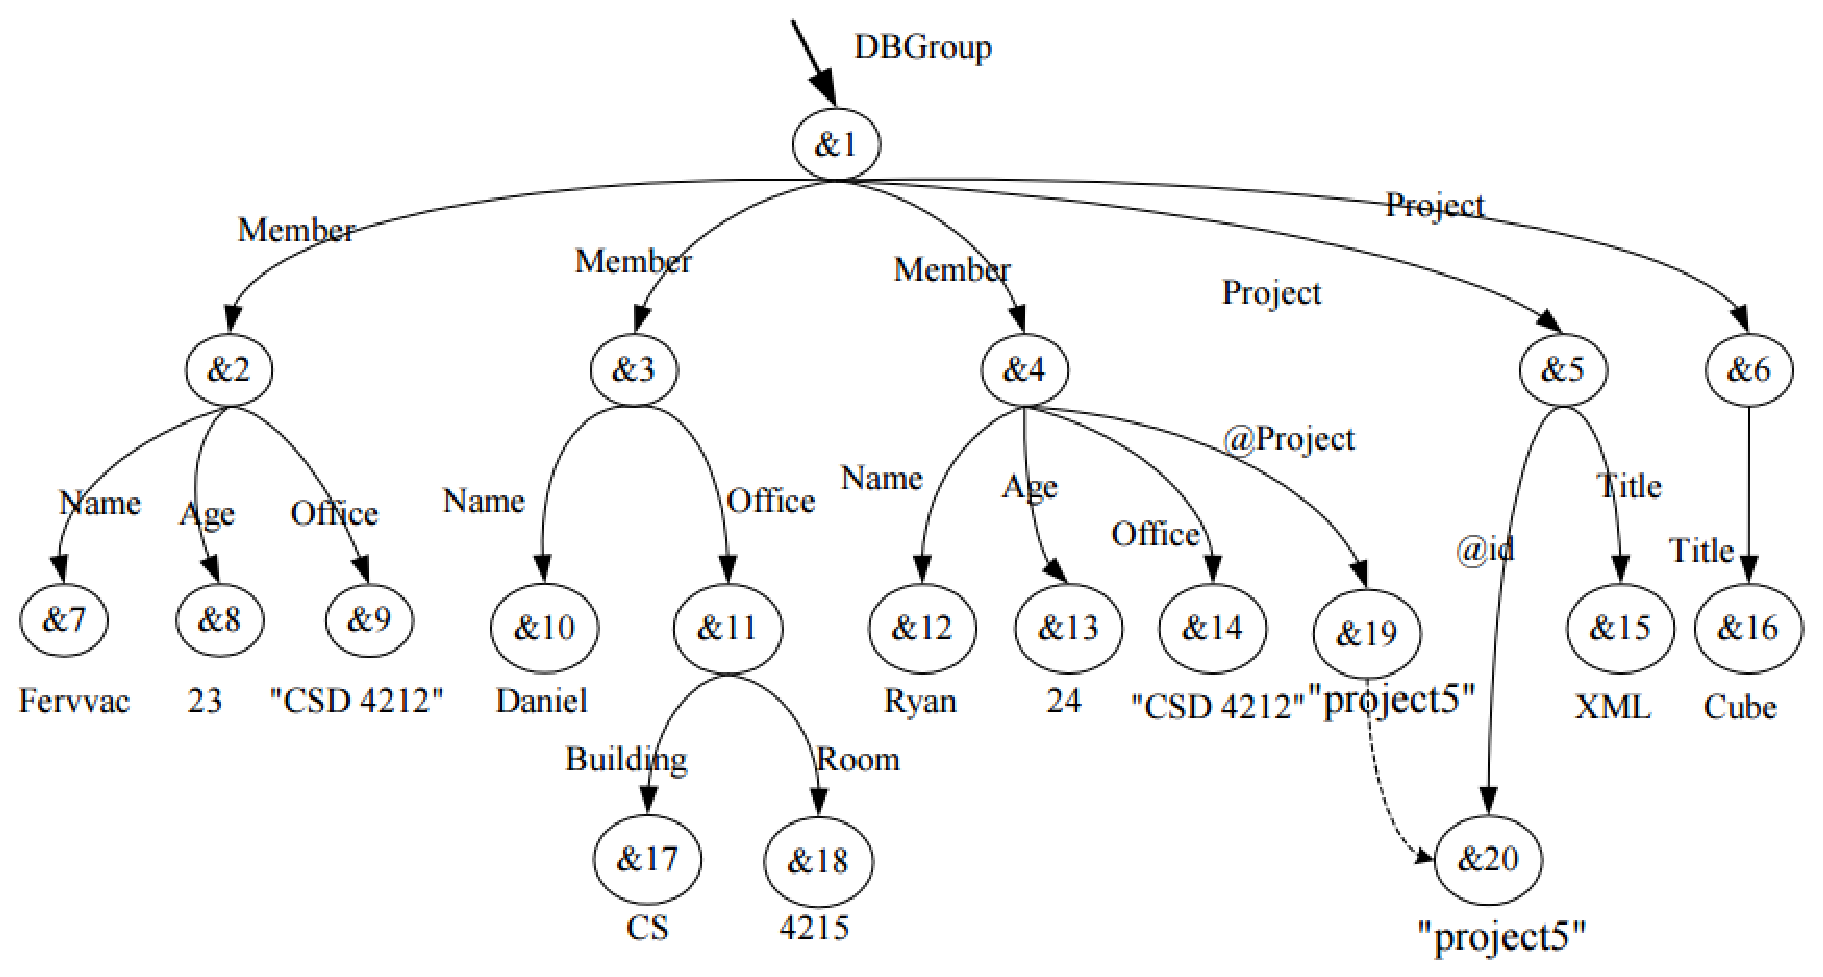
\includegraphics[height=5cm,
    angle=0]{./images/XML_graph.eps}}
\caption{A data graph for a small XML document}
\label{fig:XML_graph}
\end{figure}


The problem of storage model design for storing
XML data becomes a database schema design
problem, which can be classified into 2 categories:
\begin{itemize}
  \item {\bf structure-mapping approach} 
  
Here, the design of database schema is based on the understanding of DTD
(Document Type Descriptor) that describes the structure of XML documents.
  
  \item {\bf model-mapping approach}: 
  \begin{itemize}
    \item edge-oriented: Edge, Monet, XParent (Sect.\ref{sec:XParent}).
    
    Monet is different from the other twos; as Monet did not use a fixed schema.
    
    \item node-oriented: XRel
  
  There is no edge information explicitly maintained in this schema.
  \end{itemize}
  
Here, a fixed database schema is used to store any XML documents without
assistance of DTD,
\end{itemize}



\subsection{Edge}
\label{sec:Edge}

Edge approach uses a single table name Edge
\begin{verbatim}
Edge(Source, Ordinal, Target, Label, Flag, Value)
\end{verbatim}
to store both the label edge and data edge 
\begin{equation*}
(l_i, e_{i-1},e_i)
\end{equation*}


\subsection{Monet}
\label{sec:Monet}

Monet is a variant of Edge approach (Sect.\ref{sec:Edge}).
With Monet, all the tables are smaller. But the number of tables is huge,
because it needs to create a table for each distinctive label-path.

\subsection{XRel}
\label{sec:XRel}

XRel stores XML data graphs in four tables. They are Path, Element, Text, and
Attribute.
\begin{verbatim}
Path(PathID, Pathexp)
Element(DocId, PathID, Start, End, Ordinal)
Text(DocId, PathID, Start, End, Value)
Attribute(DocId, PathID, Start, End, Value)
\end{verbatim}
The unique feature of XRel is that no node identifiers
are needed to store XML data graphs. Instead, start
and end positions are used, which is denoted as a {\bf region}.


\subsection{XParent}
\label{sec:XParent}

It adopts the data model of XPath (Sect.\ref{sec:XPath}) to represent
XML documents.
XPath data model models XML documents as an
ordered tree using 7 types of nodes, namely, root,
element, text, attribute, namespace, processinginstruction
and comment.

XParent uses four types: root, element, text and attribute.
XParent is a four table database schema, LabelPath, DataPath, Element and Data
as follows
\begin{verbatim}
LabelPath(ID, Len, Path)
DataPath(Pid, Cid)
Element(PathID, Did, Ordinal)
Data(PathID, Did, Ordinal, Value)

\end{verbatim}

It is (a) a four table schema; b) it explicitly maintains both labelpaths
(sequences of element tags) and data-paths (sequences of elements) in two separate but
interrelated tables. The label-paths give a global view on the XML documents
stored in the database management system. As for the data-paths, two formats are
considered. The first keeps parent-child relationships.
The second further materializes it by maintaining ancestor-descendant
relationships. We call them path materialization.

